\section{Results}
\label{sec:results}

The numerical results for the problem described in Section \ref{sec:requests} are reported in the following.

\begin{figure}[H]
    \centering
    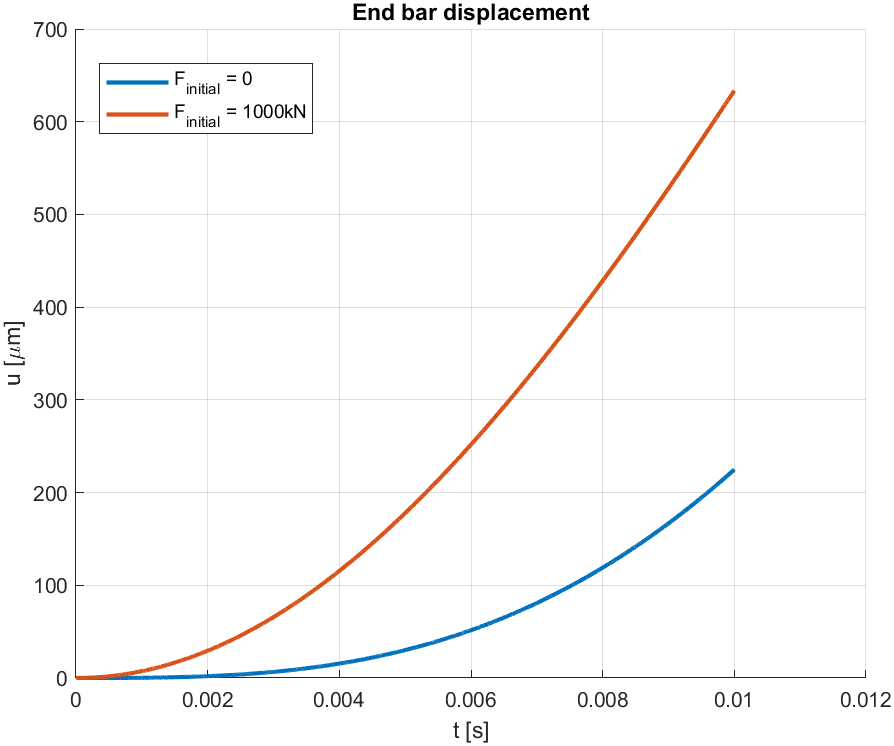
\includegraphics[width=.8\textwidth]{img/end_bar_displacement}
    \caption{Displacement of the right end of the bar vs. time}
    \label{fig:final_displacement}
\end{figure}

In Figure \ref{fig:final_displacement} we can observe a comparison between the situation in which the initial load is $F_{initial} = 0$ and linearly increased till $F_{final} = 1000kN$, and the situation in which $F_{initial} = F_{final} = 1000kN$.

In both the situation we can appreciate how the inertia of the bar is able to absorb the initial load.
